
%% bare_jrnl.tex
%% V1.4a
%% 2014/09/17
%% by Michael Shell
%% see http://www.michaelshell.org/
%% for current contact information.
%%
%% This is a skeleton file demonstrating the use of IEEEtran.cls
%% (requires IEEEtran.cls version 1.8a or later) with an IEEE
%% journal paper.
%%
%% Support sites:
%% http://www.michaelshell.org/tex/ieeetran/
%% http://www.ctan.org/tex-archive/macros/latex/contrib/IEEEtran/
%% and
%% http://www.ieee.org/

%%*************************************************************************
%% Legal Notice:
%% This code is offered as-is without any warranty either expressed or
%% implied; without even the implied warranty of MERCHANTABILITY or
%% FITNESS FOR A PARTICULAR PURPOSE! 
%% User assumes all risk.
%% In no event shall IEEE or any contributor to this code be liable for
%% any damages or losses, including, but not limited to, incidental,
%% consequential, or any other damages, resulting from the use or misuse
%% of any information contained here.
%%
%% All comments are the opinions of their respective authors and are not
%% necessarily endorsed by the IEEE.
%%
%% This work is distributed under the LaTeX Project Public License (LPPL)
%% ( http://www.latex-project.org/ ) version 1.3, and may be freely used,
%% distributed and modified. A copy of the LPPL, version 1.3, is included
%% in the base LaTeX documentation of all distributions of LaTeX released
%% 2003/12/01 or later.
%% Retain all contribution notices and credits.
%% ** Modified files should be clearly indicated as such, including  **
%% ** renaming them and changing author support contact information. **
%%
%% File list of work: IEEEtran.cls, IEEEtran_HOWTO.pdf, bare_adv.tex,
%%                    bare_conf.tex, bare_jrnl.tex, bare_conf_compsoc.tex,
%%                    bare_jrnl_compsoc.tex, bare_jrnl_transmag.tex
%%*************************************************************************


% *** Authors should verify (and, if needed, correct) their LaTeX system  ***
% *** with the testflow diagnostic prior to trusting their LaTeX platform ***
% *** with production work. IEEE's font choices and paper sizes can       ***
% *** trigger bugs that do not appear when using other class files.       ***                          ***
% The testflow support page is at:
% http://www.michaelshell.org/tex/testflow/



\documentclass[journal]{IEEEtran}
%
% If IEEEtran.cls has not been installed into the LaTeX system files,
% manually specify the path to it like:
% \documentclass[journal]{../sty/IEEEtran}





% Some very useful LaTeX packages include:
% (uncomment the ones you want to load)


% *** MISC UTILITY PACKAGES ***
%
%\usepackage{ifpdf}
% Heiko Oberdiek's ifpdf.sty is very useful if you need conditional
% compilation based on whether the output is pdf or dvi.
% usage:
% \ifpdf
%   % pdf code
% \else
%   % dvi code
% \fi
% The latest version of ifpdf.sty can be obtained from:
% http://www.ctan.org/tex-archive/macros/latex/contrib/oberdiek/
% Also, note that IEEEtran.cls V1.7 and later provides a builtin
% \ifCLASSINFOpdf conditional that works the same way.
% When switching from latex to pdflatex and vice-versa, the compiler may
% have to be run twice to clear warning/error messages.






% *** CITATION PACKAGES ***
%
\usepackage{cite}
% cite.sty was written by Donald Arseneau
% V1.6 and later of IEEEtran pre-defines the format of the cite.sty package
% \cite{} output to follow that of IEEE. Loading the cite package will
% result in citation numbers being automatically sorted and properly
% "compressed/ranged". e.g., [1], [9], [2], [7], [5], [6] without using
% cite.sty will become [1], [2], [5]--[7], [9] using cite.sty. cite.sty's
% \cite will automatically add leading space, if needed. Use cite.sty's
% noadjust option (cite.sty V3.8 and later) if you want to turn this off
% such as if a citation ever needs to be enclosed in parenthesis.
% cite.sty is already installed on most LaTeX systems. Be sure and use
% version 5.0 (2009-03-20) and later if using hyperref.sty.
% The latest version can be obtained at:
% http://www.ctan.org/tex-archive/macros/latex/contrib/cite/
% The documentation is contained in the cite.sty file itself.






% *** GRAPHICS RELATED PACKAGES ***
%
\ifCLASSINFOpdf
  \usepackage[pdftex]{graphicx}
  % declare the path(s) where your graphic files are
  \graphicspath{{../pdf/}{../jpeg/}}
  % and their extensions so you won't have to specify these with
  % every instance of \includegraphics
  \DeclareGraphicsExtensions{.pdf,.jpeg,.png}
\else
  % or other class option (dvipsone, dvipdf, if not using dvips). graphicx
  % will default to the driver specified in the system graphics.cfg if no
  % driver is specified.
  % \usepackage[dvips]{graphicx}
  % declare the path(s) where your graphic files are
  % \graphicspath{{../eps/}}
  % and their extensions so you won't have to specify these with
  % every instance of \includegraphics
  % \DeclareGraphicsExtensions{.eps}
\fi
% graphicx was written by David Carlisle and Sebastian Rahtz. It is
% required if you want graphics, photos, etc. graphicx.sty is already
% installed on most LaTeX systems. The latest version and documentation
% can be obtained at: 
% http://www.ctan.org/tex-archive/macros/latex/required/graphics/
% Another good source of documentation is "Using Imported Graphics in
% LaTeX2e" by Keith Reckdahl which can be found at:
% http://www.ctan.org/tex-archive/info/epslatex/
%
% latex, and pdflatex in dvi mode, support graphics in encapsulated
% postscript (.eps) format. pdflatex in pdf mode supports graphics
% in .pdf, .jpeg, .png and .mps (metapost) formats. Users should ensure
% that all non-photo figures use a vector format (.eps, .pdf, .mps) and
% not a bitmapped formats (.jpeg, .png). IEEE frowns on bitmapped formats
% which can result in "jaggedy"/blurry rendering of lines and letters as
% well as large increases in file sizes.
%
% You can find documentation about the pdfTeX application at:
% http://www.tug.org/applications/pdftex





% *** MATH PACKAGES ***
%
\usepackage[cmex10]{amsmath}
% A popular package from the American Mathematical Society that provides
% many useful and powerful commands for dealing with mathematics. If using
% it, be sure to load this package with the cmex10 option to ensure that
% only type 1 fonts will utilized at all point sizes. Without this option,
% it is possible that some math symbols, particularly those within
% footnotes, will be rendered in bitmap form which will result in a
% document that can not be IEEE Xplore compliant!
%
% Also, note that the amsmath package sets \interdisplaylinepenalty to 10000
% thus preventing page breaks from occurring within multiline equations. Use:
%\interdisplaylinepenalty=2500
% after loading amsmath to restore such page breaks as IEEEtran.cls normally
% does. amsmath.sty is already installed on most LaTeX systems. The latest
% version and documentation can be obtained at:
% http://www.ctan.org/tex-archive/macros/latex/required/amslatex/math/


\usepackage{amsthm}


% *** SPECIALIZED LIST PACKAGES ***
%
%\usepackage{algorithmic}
% algorithmic.sty was written by Peter Williams and Rogerio Brito.
% This package provides an algorithmic environment fo describing algorithms.
% You can use the algorithmic environment in-text or within a figure
% environment to provide for a floating algorithm. Do NOT use the algorithm
% floating environment provided by algorithm.sty (by the same authors) or
% algorithm2e.sty (by Christophe Fiorio) as IEEE does not use dedicated
% algorithm float types and packages that provide these will not provide
% correct IEEE style captions. The latest version and documentation of
% algorithmic.sty can be obtained at:
% http://www.ctan.org/tex-archive/macros/latex/contrib/algorithms/
% There is also a support site at:
% http://algorithms.berlios.de/index.html
% Also of interest may be the (relatively newer and more customizable)
% algorithmicx.sty package by Szasz Janos:
% http://www.ctan.org/tex-archive/macros/latex/contrib/algorithmicx/




% *** ALIGNMENT PACKAGES ***
%
%\usepackage{array}
% Frank Mittelbach's and David Carlisle's array.sty patches and improves
% the standard LaTeX2e array and tabular environments to provide better
% appearance and additional user controls. As the default LaTeX2e table
% generation code is lacking to the point of almost being broken with
% respect to the quality of the end results, all users are strongly
% advised to use an enhanced (at the very least that provided by array.sty)
% set of table tools. array.sty is already installed on most systems. The
% latest version and documentation can be obtained at:
% http://www.ctan.org/tex-archive/macros/latex/required/tools/


% IEEEtran contains the IEEEeqnarray family of commands that can be used to
% generate multiline equations as well as matrices, tables, etc., of high
% quality.




% *** SUBFIGURE PACKAGES ***
%\ifCLASSOPTIONcompsoc
%  \usepackage[caption=false,font=normalsize,labelfont=sf,textfont=sf]{subfig}
%\else
%  \usepackage[caption=false,font=footnotesize]{subfig}
%\fi
% subfig.sty, written by Steven Douglas Cochran, is the modern replacement
% for subfigure.sty, the latter of which is no longer maintained and is
% incompatible with some LaTeX packages including fixltx2e. However,
% subfig.sty requires and automatically loads Axel Sommerfeldt's caption.sty
% which will override IEEEtran.cls' handling of captions and this will result
% in non-IEEE style figure/table captions. To prevent this problem, be sure
% and invoke subfig.sty's "caption=false" package option (available since
% subfig.sty version 1.3, 2005/06/28) as this is will preserve IEEEtran.cls
% handling of captions.
% Note that the Computer Society format requires a larger sans serif font
% than the serif footnote size font used in traditional IEEE formatting
% and thus the need to invoke different subfig.sty package options depending
% on whether compsoc mode has been enabled.
%
% The latest version and documentation of subfig.sty can be obtained at:
% http://www.ctan.org/tex-archive/macros/latex/contrib/subfig/




% *** FLOAT PACKAGES ***
%
%\usepackage{fixltx2e}
% fixltx2e, the successor to the earlier fix2col.sty, was written by
% Frank Mittelbach and David Carlisle. This package corrects a few problems
% in the LaTeX2e kernel, the most notable of which is that in current
% LaTeX2e releases, the ordering of single and double column floats is not
% guaranteed to be preserved. Thus, an unpatched LaTeX2e can allow a
% single column figure to be placed prior to an earlier double column
% figure. The latest version and documentation can be found at:
% http://www.ctan.org/tex-archive/macros/latex/base/


%\usepackage{stfloats}
% stfloats.sty was written by Sigitas Tolusis. This package gives LaTeX2e
% the ability to do double column floats at the bottom of the page as well
% as the top. (e.g., "\begin{figure*}[!b]" is not normally possible in
% LaTeX2e). It also provides a command:
%\fnbelowfloat
% to enable the placement of footnotes below bottom floats (the standard
% LaTeX2e kernel puts them above bottom floats). This is an invasive package
% which rewrites many portions of the LaTeX2e float routines. It may not work
% with other packages that modify the LaTeX2e float routines. The latest
% version and documentation can be obtained at:
% http://www.ctan.org/tex-archive/macros/latex/contrib/sttools/
% Do not use the stfloats baselinefloat ability as IEEE does not allow
% \baselineskip to stretch. Authors submitting work to the IEEE should note
% that IEEE rarely uses double column equations and that authors should try
% to avoid such use. Do not be tempted to use the cuted.sty or midfloat.sty
% packages (also by Sigitas Tolusis) as IEEE does not format its papers in
% such ways.
% Do not attempt to use stfloats with fixltx2e as they are incompatible.
% Instead, use Morten Hogholm'a dblfloatfix which combines the features
% of both fixltx2e and stfloats:
%
% \usepackage{dblfloatfix}
% The latest version can be found at:
% http://www.ctan.org/tex-archive/macros/latex/contrib/dblfloatfix/




%\ifCLASSOPTIONcaptionsoff
%  \usepackage[nomarkers]{endfloat}
% \let\MYoriglatexcaption\caption
% \renewcommand{\caption}[2][\relax]{\MYoriglatexcaption[#2]{#2}}
%\fi
% endfloat.sty was written by James Darrell McCauley, Jeff Goldberg and 
% Axel Sommerfeldt. This package may be useful when used in conjunction with 
% IEEEtran.cls'  captionsoff option. Some IEEE journals/societies require that
% submissions have lists of figures/tables at the end of the paper and that
% figures/tables without any captions are placed on a page by themselves at
% the end of the document. If needed, the draftcls IEEEtran class option or
% \CLASSINPUTbaselinestretch interface can be used to increase the line
% spacing as well. Be sure and use the nomarkers option of endfloat to
% prevent endfloat from "marking" where the figures would have been placed
% in the text. The two hack lines of code above are a slight modification of
% that suggested by in the endfloat docs (section 8.4.1) to ensure that
% the full captions always appear in the list of figures/tables - even if
% the user used the short optional argument of \caption[]{}.
% IEEE papers do not typically make use of \caption[]'s optional argument,
% so this should not be an issue. A similar trick can be used to disable
% captions of packages such as subfig.sty that lack options to turn off
% the subcaptions:
% For subfig.sty:
% \let\MYorigsubfloat\subfloat
% \renewcommand{\subfloat}[2][\relax]{\MYorigsubfloat[]{#2}}
% However, the above trick will not work if both optional arguments of
% the \subfloat command are used. Furthermore, there needs to be a
% description of each subfigure *somewhere* and endfloat does not add
% subfigure captions to its list of figures. Thus, the best approach is to
% avoid the use of subfigure captions (many IEEE journals avoid them anyway)
% and instead reference/explain all the subfigures within the main caption.
% The latest version of endfloat.sty and its documentation can obtained at:
% http://www.ctan.org/tex-archive/macros/latex/contrib/endfloat/
%
% The IEEEtran \ifCLASSOPTIONcaptionsoff conditional can also be used
% later in the document, say, to conditionally put the References on a 
% page by themselves.


\usepackage{amssymb,mathrsfs}

% *** PDF, URL AND HYPERLINK PACKAGES ***
%
%\usepackage{url}
% url.sty was written by Donald Arseneau. It provides better support for
% handling and breaking URLs. url.sty is already installed on most LaTeX
% systems. The latest version and documentation can be obtained at:
% http://www.ctan.org/tex-archive/macros/latex/contrib/url/
% Basically, \url{my_url_here}.


\providecommand{\norm}[1]{\left\|#1\right\|}
\providecommand{\abs}[1]{\left|#1\right|}
\providecommand{\span}{\text{span}}
\providecommand{\conv}{\text{conv}}
\providecommand{\rk}[1]{\text{rank}\left(#1\right)}

\newcommand*{\Resize}[1]{\resizebox{\columnwidth}{!}{$#1$}}

\newcounter{thmcount}
\renewcommand{\thethmcount}{\arabic{thmcount}}
\renewcommand{\theequation}{\arabic{section}.\arabic{equation}}
\renewcommand{\thefigure}{\arabic{section}.\Roman{figure}}


\newtheorem{thm}[thmcount]{Theorem}
\newtheorem{cor}[thmcount]{Corollary}

\theoremstyle{remark}
\newtheorem{rem}[thmcount]{Remark}

\theoremstyle{definition}
\newtheorem{defi}[thmcount]{Definition}


% *** Do not adjust lengths that control margins, column widths, etc. ***
% *** Do not use packages that alter fonts (such as pslatex).         ***
% There should be no need to do such things with IEEEtran.cls V1.6 and later.
% (Unless specifically asked to do so by the journal or conference you plan
% to submit to, of course. )


% correct bad hyphenation here
\hyphenation{op-tical net-works semi-conduc-tor}


\begin{document}
%
% paper title
% Titles are generally capitalized except for words such as a, an, and, as,
% at, but, by, for, in, nor, of, on, or, the, to and up, which are usually
% not capitalized unless they are the first or last word of the title.
% Linebreaks \\ can be used within to get better formatting as desired.
% Do not put math or special symbols in the title.
\title{State and Input Dependent Disturbances in Min-Max Model Predictive Control}
%
%
% author names and IEEE memberships
% note positions of commas and nonbreaking spaces ( ~ ) LaTeX will not break
% a structure at a ~ so this keeps an author's name from being broken across
% two lines.
% use \thanks{} to gain access to the first footnote area
% a separate \thanks must be used for each paragraph as LaTeX2e's \thanks
% was not built to handle multiple paragraphs
%

\author{Rainer~M.~Schaich,~\IEEEmembership{Member,~IEEE,}
        Mark~Cannon
\thanks{The authors are with the Department of Engineering Science, University of
Oxford, Parks Road, Oxford, OX1~3PJ, e-mail: rainer.schaich@eng.ox.ac.uk, 
mark.cannon@eng.ox.ac.uk}% <-this % stops a space
\thanks{Manuscript received April 19, 2005; revised September 17, 2014.}}

% note the % following the last \IEEEmembership and also \thanks - 
% these prevent an unwanted space from occurring between the last author name
% and the end of the author line. i.e., if you had this:
% 
% \author{....lastname \thanks{...} \thanks{...} }
%                     ^------------^------------^----Do not want these spaces!
%
% a space would be appended to the last name and could cause every name on that
% line to be shifted left slightly. This is one of those "LaTeX things". For
% instance, "\textbf{A} \textbf{B}" will typeset as "A B" not "AB". To get
% "AB" then you have to do: "\textbf{A}\textbf{B}"
% \thanks is no different in this regard, so shield the last } of each \thanks
% that ends a line with a % and do not let a space in before the next \thanks.
% Spaces after \IEEEmembership other than the last one are OK (and needed) as
% you are supposed to have spaces between the names. For what it is worth,
% this is a minor point as most people would not even notice if the said evil
% space somehow managed to creep in.



% The paper headers
\markboth{IEEE TRANSACTIONS ON AUTOMATIC CONTROL}%
{Schaich \MakeLowercase{\textit{et al.}}: \thetitle}
% The only time the second header will appear is for the odd numbered pages
% after the title page when using the twoside option.
% 
% *** Note that you probably will NOT want to include the author's ***
% *** name in the headers of peer review papers.                   ***
% You can use \ifCLASSOPTIONpeerreview for conditional compilation here if
% you desire.




% If you want to put a publisher's ID mark on the page you can do it like
% this:
%\IEEEpubid{0000--0000/00\$00.00~\copyright~2014 IEEE}
% Remember, if you use this you must call \IEEEpubidadjcol in the second
% column for its text to clear the IEEEpubid mark.



% use for special paper notices
%\IEEEspecialpapernotice{(Invited Paper)}




% make the title area
\maketitle

% As a general rule, do not put math, special symbols or citations
% in the abstract or keywords.
\begin{abstract}
The abstract goes here.
\end{abstract}

% Note that keywords are not normally used for peerreview papers.
\begin{IEEEkeywords}
IEEEtran, journal, \LaTeX, paper, template.
\end{IEEEkeywords}






% For peer review papers, you can put extra information on the cover
% page as needed:
% \ifCLASSOPTIONpeerreview
% \begin{center} \bfseries EDICS Category: 3-BBND \end{center}
% \fi
%
% For peerreview papers, this IEEEtran command inserts a page break and
% creates the second title. It will be ignored for other modes.
\IEEEpeerreviewmaketitle



\section{Introduction}
% The very first letter is a 2 line initial drop letter followed
% by the rest of the first word in caps.
% 
% form to use if the first word consists of a single letter:
% \IEEEPARstart{A}{demo} file is ....
% 
% form to use if you need the single drop letter followed by
% normal text (unknown if ever used by IEEE):
% \IEEEPARstart{A}{}demo file is ....
% 
% Some journals put the first two words in caps:
% \IEEEPARstart{T}{his demo} file is ....
% 
% Here we have the typical use of a "T" for an initial drop letter
% and "HIS" in caps to complete the first word.
\IEEEPARstart{T}{his} demo file is intended to serve as a ``starter file''
for IEEE journal papers produced under \LaTeX\ using
IEEEtran.cls version 1.8a and later.
% You must have at least 2 lines in the paragraph with the drop letter
% (should never be an issue)
I wish you the best of success.

\hfill mds
 
\hfill September 17, 2014

\section{Problem statement}

\section{Parametrically Convex sets}
In this section we discuss \emph{parametric convexity}, an attribute of sets valued maps 
(so called point-to-set maps, see e.g.~\cite{Hogan:1973}) we exploit later on to prove 
convexity of a generalised Pontryagin difference in order to 
%
\begin{defi}[Parametric Convexity]\label{def:parametric:convexity}
  Let $X\subseteq\mathbb R^d, Y\subseteq\mathbb R^n$, let $\mathscr P(Y)$ 
  denote the power set of $Y$, 
  and $\mathcal W:X\rightarrow \mathscr P(Y)$, $X\ni p\mapsto \mathcal W(p)
  \subset Y$ be a continuous point-to-set map. The map $\mathcal W$ is called 
  \emph{parametrically convex} if it satisfies
%
  \begin{equation}\label{eq:def:parametrically:convex}
  \mathcal W(\lambda p_1 + (1-\lambda)p_2)\subseteq\lambda \mathcal W(p_1) \oplus (1-\lambda) \mathcal W(p_2)
  \end{equation}
%
  for all $p_1,p_2\in X$ and $\lambda\in[0,1]$.
\end{defi}
%
Notice that Definition~\ref{def:parametric:convexity} does not require convexity of~$\mathcal W(p)$ for all
$p\in X$, we will however only treat maps~$\mathcal W$ for which $\mathcal W(p)$ is convex.


\subsection{Abstract Properties}
%
In this subsection we introduce an equivalent characterisation of parametric 
convexity that will yield some insight on the topological 
definition~\ref{def:parametric:convexity}, for this we characterise parametric
convexity in terms of the graph of the point-to-set map.
%
\begin{defi}\label{def:graph:of:map}
Let $\mathcal W:X\rightarrow \mathscr P(Y)$ be a continuous point-to-set map
such that $\mathcal W(p)$ is convex for all $p\in X$, then 
%
\[
  \mathscr G(\mathcal W) = \{(p,x) \in\mathbb R^{d+n}: x\in\mathcal W(p)\},
\]
%
denotes the \emph{graph} of $\mathcal W$,
%
\[
  \text{int}(\mathscr G(\mathcal W)) = \{(p,x) \in\mathbb R^{d+n}: \forall d\in\mathbb R^n\;\exists 
  \epsilon>0 : x+\epsilon d\in \mathcal W(p)\}
\]
%
its \emph{interior} and
%
\[
  \partial \mathscr G(\mathcal W) = \mathscr G(\mathcal W)\setminus \textup{int}(\mathscr G(\mathcal W))
\]
%
its \emph{boundary}. 
%
The \emph{orientation cone} for all $(p,x)\in\partial\mathscr G(\mathcal W)$
is given by
%
\[
  \mathcal N\mathcal W(p,x) = \{d\in\mathbb R^n: x+\epsilon d \not\in \mathcal W(p)\; \forall \epsilon>0\}.
\]
\end{defi}
%
\begin{rem}
%
Notice, that definition~\ref{def:graph:of:map} is given in terms of the \emph{set variable} $x$ rather than \emph{graph variable} $(p,x)$.
%
Furthermore, notice that the orientation cone contains all directions that 
point out of the set, hence all linear combinations thereof.
%
\end{rem}
%
We state the central theorem to connect parametric convexity of a set valued 
map $\mathcal W$ with properties of its graph $\mathscr G(\mathcal W)$.
%
\begin{thm}\label{thm:p:convexity:graph}
The map $\mathcal W$ is parametrically convex iff for all $(p_1,x_1),(p_2,x_2)\in\partial\mathscr G(\mathcal W)$
with $\mathcal N\mathcal W(p_1,x_1)\cap\mathcal N\mathcal W(p_2,x_2)\neq\emptyset$ and $p_1\neq p_2$ 
%
\begin{equation}\label{eq:graph:def:p:convexity}
\lambda (p_1,x_1) + (1-\lambda) (p_2,x_2) \not\in\textup{int} (\mathscr G(\mathcal W))
\end{equation}
%
holds for all $\lambda\in(0,1)$.
%
\end{thm}
%
\begin{proof}
%
Assume~\eqref{eq:graph:def:p:convexity} holds for $(p_1,x_1),(p_2,x_2)\in\partial\mathscr G(\mathcal W)$.
%
Then the Minkowski functional (see e.g.~\cite{Rudin:91}) yields $\mu_{\mathscr G(\mathcal W)}(\mathcal W(\lambda p_1 + (1-\lambda)p_2),
\lambda x_1+(1-\lambda)x_2)\geq1$,
i.e. all interpolation points lie either on the boundary or outside the set $\mathcal W(\lambda p_1+(1-\lambda)p_2)$
therefore the set of all possible interpolation points 
%
\[
\begin{split}
  \lambda \mathcal W(p_1)\oplus (1-\lambda)\mathcal W(p_2) = \{x:x=\lambda x_1 + (1-\lambda) x_2 \wedge\\ x_1\in\mathcal 
  W(p_1) \wedge x_2\in\mathcal W(p_2)\}
\end{split}
\]
%
contains the set $\mathcal W(\lambda p_1 + (1-\lambda)p_2)$.
%
Now assume $\mathcal W$ is parametrically convex but~\eqref{eq:graph:def:p:convexity} is not satisfied for 
some $(p_1,x_1),(p_2,x_2)\in\partial\mathscr G(\mathcal W)$ with $\mathcal N\mathcal W(p_1,x_1)\cap\mathcal 
N\mathcal W(p_2,x_2)\neq\emptyset$, i.e. $\lambda x_1 + (1-\lambda)x_2\in\text{int}(\mathcal W(\lambda p_1 + 
(1-\lambda)p_2)$.
%
This implies that a full dimensional ball $B_\epsilon(x ) = \{y:\| 
x-y\|<\epsilon\}$
is contained in $\mathcal W(\lambda p_1 + (1-\lambda)p_2)$, i.e. $B_\epsilon(\lambda x_1 + (1-\lambda)x_2 )\subset
\mathcal W(\lambda p_1 + (1-\lambda)p_2)$ for some $\epsilon>0$.
%
Since $\mathcal N\mathcal W(p_1,x_1)\cap\mathcal N\mathcal W(p_2,x_2)\neq\emptyset$, there exist directions 
$d\in\mathcal N\mathcal W(p_1,x_1)\cap\mathcal N\mathcal W(p_2,x_2)$ which can not be represented as $d=\lambda d_1+
(1-\lambda)d_2$ with $x_1 + \epsilon d_1\in\mathcal W(p_1)$ and $x_2  + \epsilon d_2\in\mathcal W(p_2)$, however since $B_\epsilon$ is full dimensional
all directions exist, $x+\epsilon d\in\mathcal W(\lambda p_1 + (1-\lambda)p_2)$.
%
Hence, $\mathcal W$ can not be parametrically convex.
\end{proof}
%
\begin{rem}
Notice that condition~\eqref{eq:graph:def:p:convexity} is a non-convexity condition on the graph $\mathscr G(\mathcal W)$.
%
If $\mathscr G(\mathcal W)$ is strictly convex anywhere~\eqref{eq:graph:def:p:convexity} is violated and 
$\mathcal W$ can not be parametrically convex.
\end{rem}
%
\begin{cor}
%
Let $\mathcal W(p):=\{x\in\mathbb R^n: r(p,x)\leq0\}$ define a point-to-set
map with a continuous function 
$r: \mathbb R^d \times\mathbb R^n \rightarrow \mathbb R,(p,x)\mapsto r(p,x)$, 
then $\mathcal W$ is parametrically
convex iff the function $r$ is concave in $p\in\mathbb R^d$ and convex in $x\in
\mathbb R^n$.
%
\end{cor}
%
\begin{proof}
The convexity in $x\in\mathbb R^n$ is required to satisfy the requirement that $\mathcal W(p)$ is convex
for all fixed values of $p\in\mathbb R^d$. 
%
Assume that for some region $\Omega\subset\mathbb R^d$ the function $r(\cdot,x)$ is non-concave (i.e. 
strictly convex), any convex subset $\mathcal C\subseteq\Omega$ will hence be such that $\mathscr 
G(\mathcal W)\vert_{\mathcal C}$ is a convex set.
%
In particular all lines between all $(p_1,x_1),(p_2,x_2)\in \partial\mathscr G(\mathcal W)\vert_{\mathcal C}$ will satisfy
$\lambda (p_1,x_1) + (1-\lambda) (p_2,x_2) \in\textup{int} (\mathscr G(\mathcal W))\vert_{\mathcal C}$ since
$\mathscr G(\mathcal W)\vert_{\mathcal C}$ is strictly convex in $p$.
%
This implies that $r(\cdot,x)$ can not be non-concave in any non-trivial set $\Omega\subseteq\mathbb R^d$ and still
be parametrically convex.
\end{proof}
%
\begin{cor}\label{thm:polytopic:set:not:p:convex}
The polytopic parametric set valued map $\mathcal W(p):=\{x: a_i x + b_i p\leq c_i \forall i\leq m\}$ is not parametrically convex for 
any non-trivial matrix $B$.
\end{cor}
%
\begin{proof}
The graph $\mathscr G(\mathcal W)$ is given by
%
\begin{equation*}
	\mathscr G(\mathcal W) = \{(p,x):a_i x + b_i p\leq c_i \forall i\leq m\}
\end{equation*}
%
and hence is a convex set and violates Theorem~\ref{thm:p:convexity:graph}.
\end{proof}
%
\begin{cor}\label{thm:p:convexity:PWA:set:constant:num:verts}
The non-degenerate piecewise affine polytopic parametric point-to-set valued map 
%
\begin{equation}\label{eq:definition:PWA:polytopic:set:general}
  \mathcal W(p) := \left\{x: a_i x \leq \max_{k\leq l}\{b_{i,k} + C_{i,k}p\},i\leq m\right\}
\end{equation}
%
is parametrically convex iff the number of vertices $v_\kappa(p)$ and rays $r_\eta(p)$ is constant.
\end{cor}
%
\begin{proof}
For clarity this proof is divided in 3 parts:
\begin{enumerate}
\item Notice that $h_i(p) = \max_{k\leq l} \{b_{i,k} + C_{i,k}p\}$ is a multi-parametric linear program (mpLP),
its solution is a piecewise affine function $h_i(p) = b_{i,k^\ast_i} + C_{i,k^\ast_i}p$ where $k^\ast_i(p)$ is constant
inside a polytopic complex, see e.g.~\cite{spjotvold:2005}.
%
That means that there exists a finite polyhedral partitioning $\mathbb R^d = \bigcup_{j\leq t} \mathcal P_j$ with convex polyhedra 
$\mathcal P_j$ such that ${\bf{k}}^\ast\vert_{\mathcal P_j} = (k_1^\ast,\dots,k_m^\ast) = const$.
%
A standard degeneracy assumption is that in neighbouring partitions ${\bf{k}}^\ast\vert_{\mathcal P_{j_1}}$ and 
${\bf{k}}^\ast\vert_{\mathcal P_{j_2}}$ differ in exactly one element.
%
This partitioning implies that the graph $\mathscr G(\mathcal W)$ is given as a finite union of polyhedra
%
\begin{equation*}
  \mathscr G(\mathcal W) = \bigcup_{j\leq t} \left\{x: a_i x \leq b_{i,k_i^\ast} + C_{i,k_i^\ast}p,i\leq m
  \right\}\bigr\vert_{\mathcal P_{j}}
\end{equation*}
%
But this implies that if the number of vertices or rays changes inside any partition $\mathcal P_j$ then $\mathscr
G(\mathcal W)\vert_{\mathcal P_j}$ is a strictly convex polyhedron and corollary~\ref{thm:polytopic:set:not:p:convex} applies.
%
\item Our attention hence is concentrated to the boundaries of the partitions $\mathcal P_j$.
%
These are the points $\mathcal P_{j_1} \cap \mathcal P_{j_2}$ where some mpLP changes its solution, i.e. 
$\left(b_{i,k_i^\ast} + C_{i,k_{j_1}^\ast} p\right)\big\vert_{\mathcal P_{j_1}} = 
\left(b_{i,k_{j_2}^\ast} + C_{i,k_{j_2}^\ast} p\right)\big\vert_{\mathcal P_{j_2}}$.
%
Notice that a vertex $v_\kappa(p)$ is given by \emph{active} and \emph{inactive} inequalities, i.e. $\mathcal A_\kappa(p)$ and
$\mathcal I_\kappa(p) = \{1,\dots,m\}\setminus\mathcal A_\kappa(p)$ respectively.
%
\begin{equation*}\begin{split}
  a_i v_\kappa(p) &= b_{i,k_i^\ast} + C_{i,k_i^\ast} p \quad\forall i\in\mathcal A_\kappa(p)\\
  a_i v_\kappa(p) &< b_{i,k_i^\ast} + C_{i,k_i^\ast} p \quad\forall i\in\mathcal I_\kappa(p)
\end{split}\end{equation*}
%
In order for the number of vertices to change, there must be a hyperplane $fp=g$, such that the number of vertices for $fp<g$ is 
$N$ and for $fp>g$ is at least $N+1$.
%
It follows from the previous discussion that $\{p:fp=g\} = \textup{aff}\{\mathcal P_{j_1}\cap\mathcal P_{j_2}\}$ for some $j_1\neq j_2$.
%
For vertices $v_{\kappa_1}(p)$ and $v_{\kappa_2}(p)$ to merge the index sets $\mathcal A_{\kappa_1}(p)$ and 
$\mathcal A_{\kappa_2}(p)$ have to differ in only one 
element, i.e. $\mathcal A_{\kappa_1}(p) = \mathcal J\cup \{s\}$ and $\mathcal A_{\kappa_2}(p) = \mathcal J\cup\{u\}$ for $fp>g$.
%
Furthermore, for $p$ with $fp\leq g$ we have $v_{\kappa_1}(p)=v_{\kappa_2}(p)$, this implies $\mathcal A_{\kappa_1}(p) = 
\mathcal A_{\kappa_2}(p)$.
%
Since only one alteration of the active index set is considered (due to non-degeneracy assumptions), the active set 
$\mathcal A_{\kappa_1}(p) = \mathcal A_{\kappa_2}(p) = \mathcal J \cup \{s,u\}$.
%
Hence on the hyperplane $fp=g$ both, the maximising index ${\bf{k}}^\ast(p)$ and the active index sets $\mathcal A_{\kappa_1}(p)$ 
and $\mathcal A_{\kappa_2}(p)$ change, which is means the problem is degenerate.
%
\item In order for the degenerate graph $\mathscr G(\mathcal W)$ to be parametrically convex the overdetermined 
vertex $v_{\kappa_1}(p)=v_{\kappa_2}(p)$ have to be identical, in particular their dependence on $p$ has to be identical.
%
This can be expressed with the implicit function theorem:
%
\begin{equation*}\begin{split}
  \frac{d}{dp}\left(  A_{\mathcal J\cup \{s\}} v_{\kappa_1}(p) - b_{\mathcal J\cup \{s\}} - C_{\mathcal J\cup \{s\},{\bf{k}}^\ast} p\right) &= 0\\
  \frac{d}{dp}\left(  A_{\mathcal J\cup \{u\}} v_{\kappa_2}(p) - b_{\mathcal J\cup \{u\}} - C_{\mathcal J\cup \{u\},{\bf{k}}^\ast} p\right) &= 0
\end{split}\end{equation*}
%
which leads to 
%
\begin{equation*}\begin{split}
  A_{\mathcal J\cup \{s\}} \frac{dv_{\kappa}}{dp} &= C_{\mathcal J\cup \{s\},{\bf{k}}^\ast}\\
  A_{\mathcal J\cup \{u\}} \frac{dv_{\kappa}}{dp} &= C_{\mathcal J\cup \{u\},{\bf{k}}^\ast}
\end{split}\end{equation*}
%
since we can assume that the inequalities are non-redundant for some right hand side, we obtain that 
%
\begin{equation}\label{eq:derivative:condition:on:index:sets}
  \frac{dv_\kappa}{dp} = A_{\mathcal J\cup \{s\}}^{-1}C_{\mathcal J\cup \{s\},{\bf{k}}^\ast} = 
  A_{\mathcal J\cup \{u\}}^{-1}C_{\mathcal J\cup \{u\},{\bf{k}}^\ast}
\end{equation}
%
has to hold for the degenerate graph to remain parametrically convex.
%
Notice that~\eqref{eq:derivative:condition:on:index:sets} is again a degenerate condition, since arbitrarily small perturbations
will produce different behaviour.
\end{enumerate}
\end{proof}
%
\begin{rem}
Corollary~\ref{thm:p:convexity:PWA:set:constant:num:verts} is essential for numerical examples, as it can be reformulated to:
%
The set valued map defined by~\eqref{eq:definition:PWA:polytopic:set:general} is non-degenerate and parametrically convex iff 
it has a constant number of vertices throughout the parameter space~$X$.
%
Since the map is continuous it is sufficient to verify this at the vertices of the parameter space.
%
\end{rem}
%
In order to determine MRPI sets we need to be able to calculate the Pontryagin difference between sets, hence we introduce
the following.
%
\begin{defi}[Parametric Pontryagin Difference]\label{def:parametric:pontryagin:difference}
  Let $S\subseteq X$ and let $\mathcal W:X\to\mathscr P(X)$ be a continuous point-to-set map such that
  $\mathcal W(p)$ is convex for all $p\in X$, then the \emph{parametric Pontryagin difference} 
  $S\ominus \mathcal W(S)$ is 
  \begin{equation}\label{eq:definition:parametric:pontryagin:difference}
    S\ominus \mathcal W(S) = \left\{x\in X: \{x\} \oplus \mathcal W(x)\subseteq S\right\},
  \end{equation}
  where $\mathcal W(S)$ denotes the image of $S$ under the map $\mathcal W$. 
\end{defi}
%
For the parametric Pontryagin difference of a convex set and a parametrically convex map we 
have the following result.
%
\begin{thm}\label{thm:convexity:of:pontryagin:difference}
  Let $S\subseteq X$ be a convex set and let $\mathcal W:X\rightarrow\mathscr P(X)$ be a parametrically convex point-to-set
  map such that $\mathcal W(p)$ is convex for all $p\in X$, then $S\ominus \mathcal W(S)$ is convex.
\end{thm}
%
\begin{proof}
To prove the convexity of $ Z :=  S\ominus \mathcal W( S)$ we pick any $z_1,z_2\in Z$, then
by definition of the parametric Pontryagin difference, we have
%
\begin{equation}
  \{z_i\} \oplus \mathcal W(z_i) \subseteq S,\; i=1,2.
\end{equation}
%
To see that $ Z$ is convex we show that line segments between
all possible $z_1$ and $z_2$ are subsets of $ Z$, i.e.~for all $\lambda \in [0,1]$,
\begin{equation}
\begin{aligned}
  \{ \lambda z_1 + (1-&\lambda)z_2
  \}\oplus \mathcal W\left( \lambda z_1 + (1-\lambda)z_2\right)\\
  \subseteq&\left\{ \lambda z_1 + (1-\lambda)z_2
  \right\}\oplus \lambda \mathcal W(z_1) \oplus (1-\lambda)
  \mathcal W(z_2)\\
  \subseteq &\lambda\underbrace{(\{z_1\}\oplus \mathcal W(z_1))}_{\subseteq S}\oplus
  (1-\lambda)\underbrace{(\{z_2\}\oplus \mathcal W(z_2))}_{\subseteq S}\\
  \subseteq& Z
\end{aligned}
\end{equation}
%
where the last inclusion follows from the convexity of $\mathcal S$.
\end{proof}
%
Theorem~\ref{thm:convexity:of:pontryagin:difference} only gives us the convexity of the parametric
Pontryagin difference, in the following we will see that the parametric Pontryagin difference between
a polyhedral set and a piecewise affine polytopic parametric set is polyhedral itself.

\subsection{Maximal Robust Positive Invariant Sets}



\subsection{Example I}

\section{Recursive Multi-Parametric Quadratic Programming to Solve Min-Max Programs}

\section{Solving Min-Max Programs}

\section{Example II}

% needed in second column of first page if using \IEEEpubid
%\IEEEpubidadjcol


% An example of a floating figure using the graphicx package.
% Note that \label must occur AFTER (or within) \caption.
% For figures, \caption should occur after the \includegraphics.
% Note that IEEEtran v1.7 and later has special internal code that
% is designed to preserve the operation of \label within \caption
% even when the captionsoff option is in effect. However, because
% of issues like this, it may be the safest practice to put all your
% \label just after \caption rather than within \caption{}.
%
% Reminder: the "draftcls" or "draftclsnofoot", not "draft", class
% option should be used if it is desired that the figures are to be
% displayed while in draft mode.
%
%\begin{figure}[!t]
%\centering
%\includegraphics[width=2.5in]{myfigure}
% where an .eps filename suffix will be assumed under latex, 
% and a .pdf suffix will be assumed for pdflatex; or what has been declared
% via \DeclareGraphicsExtensions.
%\caption{Simulation results for the network.}
%\label{fig_sim}
%\end{figure}

% Note that IEEE typically puts floats only at the top, even when this
% results in a large percentage of a column being occupied by floats.


% An example of a double column floating figure using two subfigures.
% (The subfig.sty package must be loaded for this to work.)
% The subfigure \label commands are set within each subfloat command,
% and the \label for the overall figure must come after \caption.
% \hfil is used as a separator to get equal spacing.
% Watch out that the combined width of all the subfigures on a 
% line do not exceed the text width or a line break will occur.
%
%\begin{figure*}[!t]
%\centering
%\subfloat[Case I]{\includegraphics[width=2.5in]{box}%
%\label{fig_first_case}}
%\hfil
%\subfloat[Case II]{\includegraphics[width=2.5in]{box}%
%\label{fig_second_case}}
%\caption{Simulation results for the network.}
%\label{fig_sim}
%\end{figure*}
%
% Note that often IEEE papers with subfigures do not employ subfigure
% captions (using the optional argument to \subfloat[]), but instead will
% reference/describe all of them (a), (b), etc., within the main caption.
% Be aware that for subfig.sty to generate the (a), (b), etc., subfigure
% labels, the optional argument to \subfloat must be present. If a
% subcaption is not desired, just leave its contents blank,
% e.g., \subfloat[].


% An example of a floating table. Note that, for IEEE style tables, the
% \caption command should come BEFORE the table and, given that table
% captions serve much like titles, are usually capitalized except for words
% such as a, an, and, as, at, but, by, for, in, nor, of, on, or, the, to
% and up, which are usually not capitalized unless they are the first or
% last word of the caption. Table text will default to \footnotesize as
% IEEE normally uses this smaller font for tables.
% The \label must come after \caption as always.
%
%\begin{table}[!t]
%% increase table row spacing, adjust to taste
%\renewcommand{\arraystretch}{1.3}
% if using array.sty, it might be a good idea to tweak the value of
% \extrarowheight as needed to properly center the text within the cells
%\caption{An Example of a Table}
%\label{table_example}
%\centering
%% Some packages, such as MDW tools, offer better commands for making tables
%% than the plain LaTeX2e tabular which is used here.
%\begin{tabular}{|c||c|}
%\hline
%One & Two\\
%\hline
%Three & Four\\
%\hline
%\end{tabular}
%\end{table}


% Note that the IEEE does not put floats in the very first column
% - or typically anywhere on the first page for that matter. Also,
% in-text middle ("here") positioning is typically not used, but it
% is allowed and encouraged for Computer Society conferences (but
% not Computer Society journals). Most IEEE journals/conferences use
% top floats exclusively. 
% Note that, LaTeX2e, unlike IEEE journals/conferences, places
% footnotes above bottom floats. This can be corrected via the
% \fnbelowfloat command of the stfloats package.




\section{Conclusion}
The conclusion goes here.




% if have a single appendix:
%\appendix[Proof of the Zonklar Equations]
% or
%\appendix  % for no appendix heading
% do not use \section anymore after \appendix, only \section*
% is possibly needed

% use appendices with more than one appendix
% then use \section to start each appendix
% you must declare a \section before using any
% \subsection or using \label (\appendices by itself
% starts a section numbered zero.)
%


\appendices
\section{Proof of the First Zonklar Equation}
Appendix one text goes here.

% you can choose not to have a title for an appendix
% if you want by leaving the argument blank
\section{}
Appendix two text goes here.


% use section* for acknowledgment
\section*{Acknowledgment}


The authors would like to thank...


% Can use something like this to put references on a page
% by themselves when using endfloat and the captionsoff option.
\ifCLASSOPTIONcaptionsoff
  \newpage
\fi



% trigger a \newpage just before the given reference
% number - used to balance the columns on the last page
% adjust value as needed - may need to be readjusted if
% the document is modified later
%\IEEEtriggeratref{8}
% The "triggered" command can be changed if desired:
%\IEEEtriggercmd{\enlargethispage{-5in}}

% references section

% can use a bibliography generated by BibTeX as a .bbl file
% BibTeX documentation can be easily obtained at:
% http://www.ctan.org/tex-archive/biblio/bibtex/contrib/doc/
% The IEEEtran BibTeX style support page is at:
% http://www.michaelshell.org/tex/ieeetran/bibtex/
\bibliographystyle{IEEEtran}
% argument is your BibTeX string definitions and bibliography database(s)
\bibliography{IEEEabrv,MyLib}

%
% <OR> manually copy in the resultant .bbl file
% set second argument of \begin to the number of references
% (used to reserve space for the reference number labels box)
% \begin{thebibliography}{1}

% \end{thebibliography}

% biography section
% 
% If you have an EPS/PDF photo (graphicx package needed) extra braces are
% needed around the contents of the optional argument to biography to prevent
% the LaTeX parser from getting confused when it sees the complicated
% \includegraphics command within an optional argument. (You could create
% your own custom macro containing the \includegraphics command to make things
% simpler here.)
%\begin{IEEEbiography}[{\includegraphics[width=1in,height=1.25in,clip,keepaspectratio]{mshell}}]{Michael Shell}
% or if you just want to reserve a space for a photo:

\begin{IEEEbiography}[{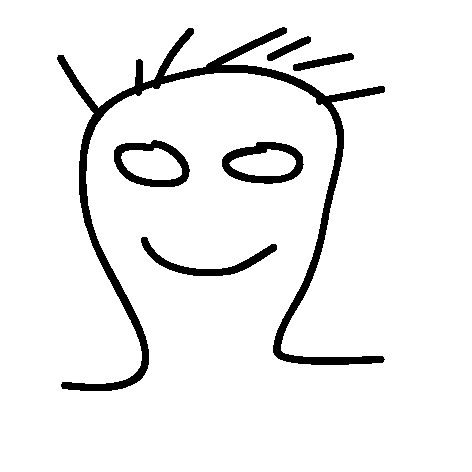
\includegraphics[width=1in,height=1.25in,clip,keepaspectratio]{face.pdf}}]{Rainer Manuel Schaich}
Biography text here.
\end{IEEEbiography}

% if you will not have a photo at all:
\begin{IEEEbiography}[{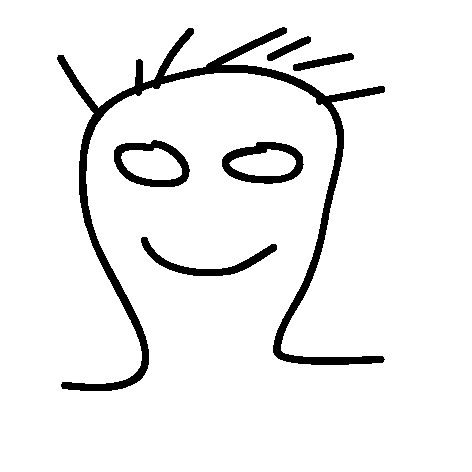
\includegraphics[width=1in,height=1.25in,clip,keepaspectratio]{face.pdf}}]{Mark Cannon}
Biography text here.
\end{IEEEbiography}

% insert where needed to balance the two columns on the last page with
% biographies
%\newpage

% You can push biographies down or up by placing
% a \vfill before or after them. The appropriate
% use of \vfill depends on what kind of text is
% on the last page and whether or not the columns
% are being equalized.

%\vfill

% Can be used to pull up biographies so that the bottom of the last one
% is flush with the other column.
%\enlargethispage{-5in}



% that's all folks
\end{document}


